\documentclass{article}
\usepackage{graphicx} % Required for inserting images
\graphicspath{ {./images/} }

\title{Project 3 Cryptography}
\author{Caden Kim, Brennan Longstreth, Riley Sikes }
\date{February 2023}

\begin{document}

\maketitle

\section{Homework 3}

\subsection{Caesar}

Ciphertext-only attack.

\subsection{Key Exchange Problem}

Alice and Bob both wish to communicate using a secret key cryptosystem. The problem with this is that they both must agree to a key that is only known to them. If anyone else gets the key, like Mallory for example, they can get send messages to Bob from Alice or vice versa. The problem is how do Alice and Bob agree on a key to use without letting it be known to Mallory or anyone else that's eavesdropping on the system.

\subsection{Public Key Attack}

Subject to a man in the middle attack.

% 4
\subsection{ADFGVX}
Decrypt: AVFFDDD ADVAXGF FXVXVGX \\

Key 2: ENCRYPT \\
\begin{center}
\begin{tabular}{ c c c c c c c }
    E & N & C & R & Y & P & T \\ [0.5ex] 
    \hline
    F & D & A & G & V & V & X \\
    D & A & V & F & G & A & V \\
    D & D & F & F & X & X & X \\
\end{tabular}
\end{center}
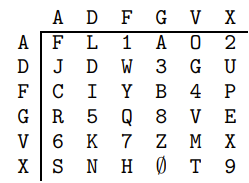
\includegraphics{Cipher}\\

So then the intermediate text is now: $$FDAGVVXDAVFGAVDDFFXXX$$
Using the permutation as shown on p. 17, the letters are as follows:
$$FD = I$$
$$AG = A$$
$$VV = M$$
$$XD = N$$
$$AV = O$$
$$FG = B$$
$$AV = O$$
$$DD = D$$
$$FF = Y$$
$$XX = 9$$
$$X = X$$
Therefore the decrypted message is: $$IAMNOBODY9X$$

\subsection{Division Algorithm}

Given integers $a$, $b$ with $b > 0$, there exists unique integers $q$, $r$ satisfying $$a = qb + r$$
$$0 \le r < b$$
We say: $q$ is the quotient\\
$b$ is the divisor\\
$r$ is the remainder\\

\subsection{Proof}
Using the division algorithm show that the cube of any integer is of the form $9k$, $9k+1$, or $9k+8$\\\\
By the division algorithm we can write any integer as $a = 9k + r$ where the possible values for $r$ are $0 < r < 9$\\\\
Observe that $a^3 = (9k + r)^3 = (9k)^3 + 3(9k)^2r + 3(9k)r^2 + r^3$\\\\
This can be simplified by pulling a nine out of everything except $r^3$ to $$9(81k^3+27k^2r+3kr^2) + r^3$$
We know the inside of the parenthesis must be an integer so now we just need to find the possible $r$ values. We know $0 < r < 9$ so we can start checking our possible values to see if they fit. 
\\\\
Case $r=0$ we get $a=9k$
\\\\
Case $r=1$ we get $a=9k+1$
\\\\
Case $r=2$ we get $a=9k+8$
\\\\
Any $r$ values greater than two we get $r^3$ values greater than eight which we can't have.
\\\\
Thus the cube of any integer is of the form $9k$, $9k+1$, or $9k+8$.

\subsection{Proof}
Using the division algorithm, show that the square of any integer is of the form $3k$ or $3k+1$
\\\\
By the division algorithm we can write any integer as $a = 3k + r$ where the possible values for $r$ are $0 < r < 3$\\\\
Observe that $a^3 = (3k + r)^2 = (3k)^2 + 6kr + r^2$\\\\
This can be simplified by pulling a three out of everything except $r^2$ to $$3(3k^2+3kr) + r^2$$
We know the inside of the parenthesis must be an integer so now we just need to find the possible $r$ values. We know $0 < r < 3$ so we can start checking our possible values to see if they fit. 
\\\\
Case $r=0$ we get $a=3k$
\\\\
Case $r=1$ we get $a=3k+1$
\\\\
Any $r$ values greater than one we get $r^2$ values greater than two which we can't have.
\\\\
Thus the square of any integer is of the form $3k$ or $3k+1$.

\subsection{Proof}
Using the result from problem 7, show that $3a^2 - 1$ is never a perfect square.
\\\\
We know from problem 7 that the square of any integer can be represented as $3k$ or $3k+1$ for some $k \in Z$
\\\\
Case 1: $a^2 = 3k$
$$3a^2 - 1 = 3(3k) - 1$$
This is equivalent to $3k - 1$ or $3k+2$ which is not one of our possible integer representations.
\\\\
Case 2: $a^2 = 3k+1$
$$3a^2 - 1 = 3(3k+1) - 1 = 9k+3-1=3(3k) +2$$
This is equivalent to $3k + 1$ or $3k-1$ which is not one of our possible integer representations.\\\\
Therefore $3a^2 - 1$ is never a perfect square.

\subsection{Euclid's Algorithm}
Find gcd$(482,1180)$
\\\\
$$1180 = 482 * 2 + 216$$
$$482 = 216 * 2 + 50$$
$$216 = 50 * 4 + 16$$
$$50 = 16 * 3 + 2$$
$$16 = 2 * 8 + 0$$
Therefore the gcd$(482,1180) = 2$

\subsection{Extended Euclid}
Let $482S + 1180T =$ gcd$(482,1180)$
\\\\
$$2 = 50 - (16 * 3)$$
$$2 = 50 - ((216 - (50*4)) * 3)$$
$$2 = 50 - ((216*3) - (50*12))$$
$$2 = 50 - (216*3) + (50*12))$$
$$2 = -(216*3) + (50*13))$$
$$2 = -(216*3) + ((482-(216*2))*13))$$
$$2 = -(216*3) + (482*13-(216*26)))$$
$$2 = (482*13)-(216*29)$$
$$2 = (482*13)-((1180 - (482*2))*29)$$
$$2 = (482*13)-((1180*29) - (482*58))$$
$$2 = (482*13)-(1180*29) + (482*58)$$
$$2 = (482*71)-(1180*29)$$

Therefore $S = 71$ and $T=-29$

\end{document}